\chapter{Evaluation}\pagestyle{fancy}\setlength{\parindent}{3em}
\label{chap:evaluation}

As I developed a processing pipeline to extract the tire-markings off images of tires, I needed a dataset. To build this dataset I took photos with a Cannon EOS 1300D that has a resolution of 5184 by 3456 pixels, but the picture was cropped around the center to 3456 by 3456 pixels so that the image would be square. The lens used is EF-S 18-55mm Canon Zoom which has diameter of 58mm. When taking pictures I used a focal length of 23 millimeters and the aperture, exposure time and ISO were kept on "auto". In the process of building the dataset, the distance from the lens to the tire's side was approximately 115 centimeters and the average exposure time was 1/93 seconds. The dataset size is of 107 images.

While capturing the images, I was careful to catch the entire wheel in the image because detecting half wheels or arcs would have proven difficult. One more adjustment I did was the camera placement in regards to the wheel's axle. I decided to be approximately in line with it in order for the wheel to appear circular in the image. If I wouldn't have done so, the tire would have had an oval shape which would not affect very much the unwrapping faze as it has some slack and it doesn't require the tire to be perfectly circular. Anyway, the outer rim of the tire doesn't have a circular shape because it is deformed at the contact point with the ground. The oval shape affects the unwrapped output like Figure \ref{fig:tire_unwrapping-unwrapped-failed}, compared to Figure \ref{fig:tire_unwrapping-unwrapped}.

By controlling the distance between the camera and the wheel, as  well as the camera position in regards to the wheel's axle, I was be able to detect the tire in the image more reliably and ensured the letters composing the tire-markings had at least 20 pixels in height.

When it comes to evaluating the running time, the system the algorithm is tested on contains an Intel i7-6700HQ CPU and 16GB of DDR4 RAM at 2133 Mega-transfers/s. The operating system is Ubuntu 20.04.4 LTS 64 bit with Linux Kernel 5.5.9-050509-generic. In measuring the time, I do not take into account the writing time to the storage media.

There are three main points in which the pipeline can be evaluated and they coincide with its steps. The first is the percentage of the dataset in which the tire could be identified and unwrapped. The second is the percentage of codes found in average on a tire and the average quantity of false positives in the regions of interest extracted. The third is the performance of the OCR in correctly recognizing the regions of interest.

\section{Evaluating the Tire Unwrapping (Stage 1)}\label{section:evaluation-tire_unwrapping}

I measured what percentage of the input images my algorithm is able to unwrap successfully. This is partially automated and partially manual. My algorithm tries to obtain the circles approximately matching to the outer and inner rims of the tire. If more circles are detected and the algorithm is not able to reduce their number to only two or not even 2 are found, the respective image will be discarded automatically. The manual part is to pass through each successfully unwrapped image and check if the wheel's center was correctly detected. If not, I will discard the image before proceeding to the next phase.

It turned out that the pipeline could identify and unwrap the tire in 86 images out of the 107 in the dataset. Out of these 86 unwrapped images, 5 were false positives that I observed while manually passing through them. So the first stage of the algorithm could find and unwrap the tire in 75.7\% of the dataset.

By performing the action of unwrapping and keeping only the tire, I succeeded in reducing the number of pixels in the image by an average of 7,139,770 pixels (59,77\% of the squared original size), the distribution of the pixel reduction count could be seen in Figure \ref{fig:pixel_count_reduced-stage1}.

This stage on the hardware configuration previously stated has an average running time of 1.39 seconds (Figure \ref{fig:running_time-stage1}). It must be noted that the IO operations with the long term storage medium are not taken into account when it comes to measuring the running time.

\begin{figure}
    \centering
    \begin{minipage}[c]{0.5\linewidth}
        \centering
        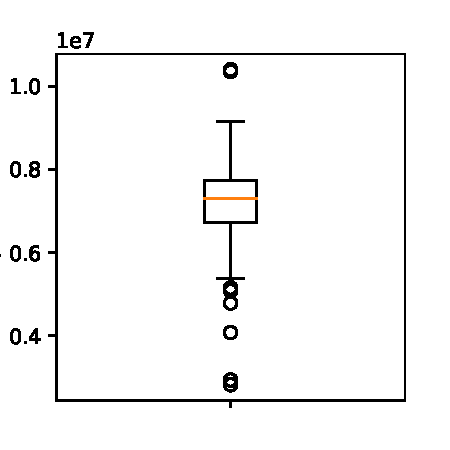
\includegraphics[height=7cm, keepaspectratio]{img/evaluation/no_of_pixels_reduced-stage1.pdf}
            \caption{No. of pixels reduced by Stage 1}
            \label{fig:pixel_count_reduced-stage1}
    \end{minipage}\hfill
    \begin{minipage}[c]{0.5\linewidth}
        \centering
        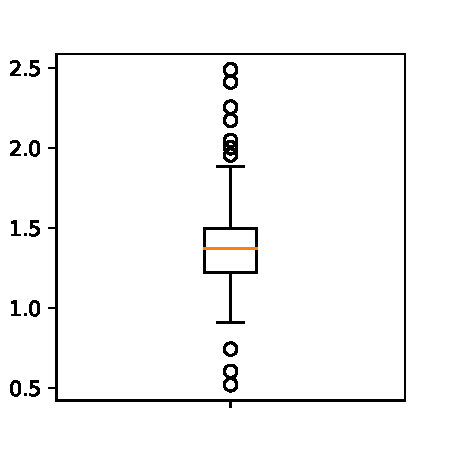
\includegraphics[height=7cm, keepaspectratio]{img/evaluation/running_time-stage1.pdf}
            \caption{Running time of Stage 1}
            \label{fig:running_time-stage1}
    \end{minipage}
\end{figure}

\section{Evaluating the Text Detection (Stage 2)}\label{section:evaluation-text_detection}

When designing the pipeline part to detect text regions, I allowed for a higher number of false positives in order to detect as many codes and text regions as possible. In the successfully unwrapped images (numbering 81) the second stage detected a total of 1623 regions of interest, out of which . Thus, the precision of this step is (36.97\%).

Before measuring the performance of detecting the tire-markings I am interested in -- the DOT code and E-mark certification --, it is needed to define a few edge cases. If the text of a marking, for example the DOT code, is split in multiple segments instead of single one, it will be considered as a valid recognition and a new metric for segmented detections will be used. If a text region is incomplete recognized, it will be considered as being valid and this will accounted by another metric for incomplete recognitions. If the past 2 cases combine, it will be considered the tire-marking is also segmented and incomplete. For example if there is the DOT code "DOT ABCD EFG 0123" and it was detected as 2 regions "OT ABCD" and "01", they will be considered as one valid recognition, one segmented recognition and one incomplete recognition. If in the detected region of interest are present other markings besides the DOT code or the E-mark, it will be accounted as a combined detection.

% TODO: sa fac inceputul paragrafului de mai jos intr-o figura sau tabel? N am idei :(

In the successfully unwrapped images (amounting to 81), 1623 zones were considered to contain text, 600 contained any kind of text (true positives) and 1023 were false positives (63.03\%). 151 identification tire-markings (DOT code and E-mark certification) were present in the unwrapped images and the algorithm successfully detected 116 (76.82\% out of all the codes) markings, out of which 16 were segmented (13.79\% out of the detected markings), 45 were incomplete (38.79\% out of the detected markings) and 24 were combined with other markings(20.68\% out of the detected markings).

To measure the performance of the pipeline in detecting only the tire identification codes and not any other text in the image, I need to consider true positives only the 116 detections and the rest of 1507 false positives. The number of false negatives is 35. I used the metrics described in the work of Afzal Godil et alia \cite{article:evaluation-metrics} to evaluate this step in the pipeline. The results are summarized in Table \ref{tab:evaluation_metrics-stage2}.

\begin{table}
    \begin{tabular}{|c|c|c|c|c|c|}
    \hline
    Metric & False Alarm Rate & Detection Rate & False Negative Rate & Precision & Recall \\ \hline
    Value  & 0.92             & 0.76           & 0.23                & 0.07      & 0.76   \\ \hline
    \end{tabular}
    \caption{Evaluation metrics for Stage 2}
    \label{tab:evaluation_metrics-stage2}
\end{table}

By finding regions of interest in the images, the space in which OCR must be performed later is reduced in average by 91.36\% of the unwrapped image size. The average running time of this stage is 4.51 seconds (Figure \ref{fig:running_time-stage2}).

\begin{figure}
    \centering
    \begin{minipage}[c]{0.5\linewidth}
        \centering
        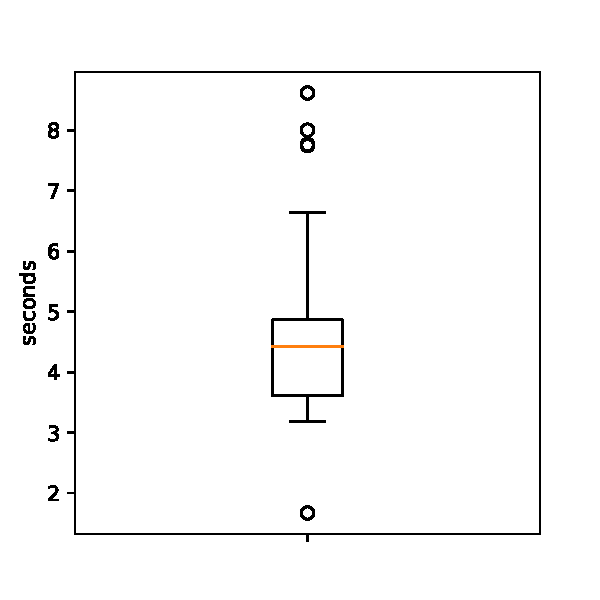
\includegraphics[height=7cm, keepaspectratio]{img/evaluation/running_time-stage2.pdf}
            \caption{Running time of Stage 2}
            \label{fig:running_time-stage2}
    \end{minipage}\hfill
\end{figure}

\section{Evaluating the Text Recognition (Stage 3)}\label{section:evaluation-ocr}

When it comes to evaluating the OCR, I will use the Character Error Rate (CER) \cite{site:evaluation-OCR-character_error_rate} metric. This will show the performance of the algorithm in recognizing the letters out of the good regions of interest, lower being better.
\[CER = \frac{S + D + I}{N}\]
Where S is \# of substitutions, D is \# of deletions, I is \# of insertions and N is \# of characters in ground truth.

I will hand pick the true positive images containing text of an acceptable image quality and discard the false positives detected at the \ref{sec:text-detection} Text Detection section stage because I have limited a limited number of credits to try out the OCR (called Read API) from Microsoft Cognitive Services \cite{site:Microsoft_Cognitive_Services}.

\begin{figure}
    \centering
    \begin{minipage}[c]{0.5\linewidth}
        \centering
        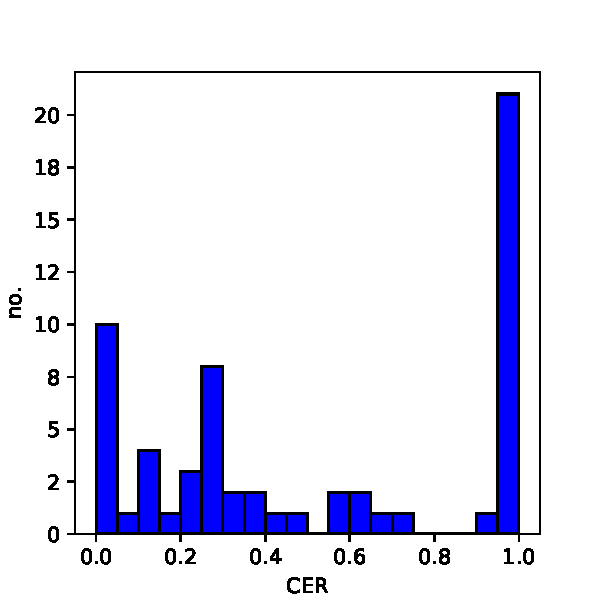
\includegraphics[height=7cm, keepaspectratio]{img/evaluation/CER_on_all-stage3.pdf}
            \caption{CER dist. on $TP\_S$}
            \label{fig:CER_on_all-stage3}
    \end{minipage}\hfill
    \begin{minipage}[c]{0.5\linewidth}
        \centering
        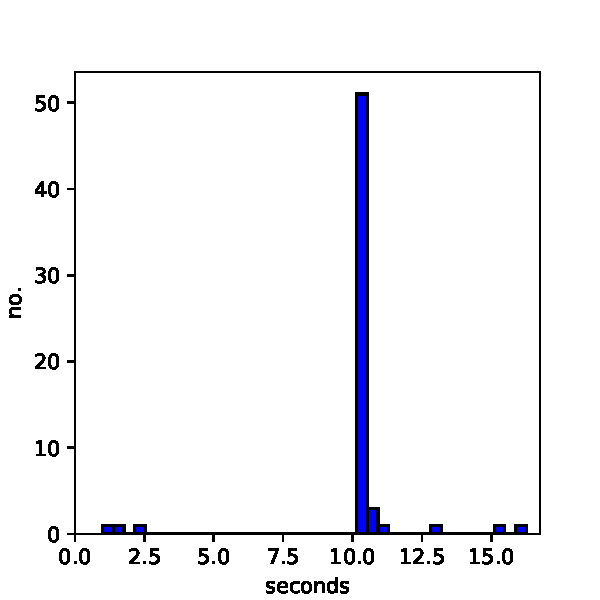
\includegraphics[height=7cm, keepaspectratio]{img/evaluation/running_time-stage3.pdf}
            \caption{Running time of Stage 3}
            \label{fig:running_time-stage3}
    \end{minipage}\hfill
\end{figure}

I have selected a subset of 61 true positives (called $TP\_S$) detected at the \ref{sec:text-detection} Text Detection stage. An interesting thing happened. If the OCR was able to find text in the image, it could recognize pretty good the characters in the image and usually almost all of it. However, there is a discrepancy in the number of characters recognized in lower quality photos or blurry ones as the OCR fails to recognize any characters. This can be observed in the distribution of CER values for the 61 true positives in Figure \ref{fig:CER_on_all-stage3} and has an average CER of 0.51. If we remove the images where no text could be recognized we get a distribution like in Figure \ref{fig:CER_on_arecognized-stage3} with an average CER of 0.26. This is a good sign that the OCR is working well on images that are not blurry or too dark (like Figure \ref{fig:text_recognition-blurry_image}) and without contrast. I also measured the CER only on the words recognized in a image from $TP\_S$ and gave a distribution like in Figure \ref{fig:CER_on_recognized_words-stage3} with an average CER of 0.20.

Measuring the running time is not a precise task as the OCR is a web service and it would depend on the network congestion and the service's load at the time. Anyhow, I still measured the time it takes from the submission of the request to the response. It resulted in an average of 10.17 seconds and as can be seen in Figure \ref{fig:running_time-stage3}, the majority of the response time values is around this value with a few outliers. This may be an artificially induced delay in the service provided by Microsoft Cognitive Services.

\begin{figure}
    \centering
    \begin{minipage}[c]{0.5\linewidth}
        \centering
        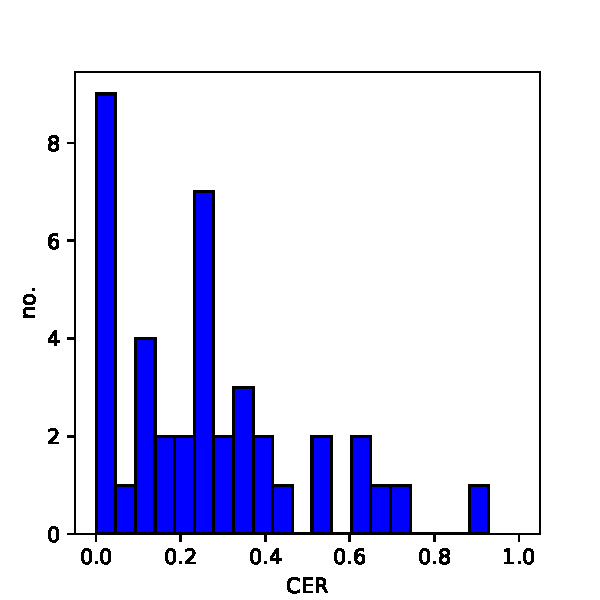
\includegraphics[height=7cm, keepaspectratio]{img/evaluation/CER_on_recognized-stage3.pdf}
            \caption{CER dist. on any recognized $TP\_S$}
            \label{fig:CER_on_arecognized-stage3}
    \end{minipage}\hfill
    \begin{minipage}[c]{0.5\linewidth}
        \centering
        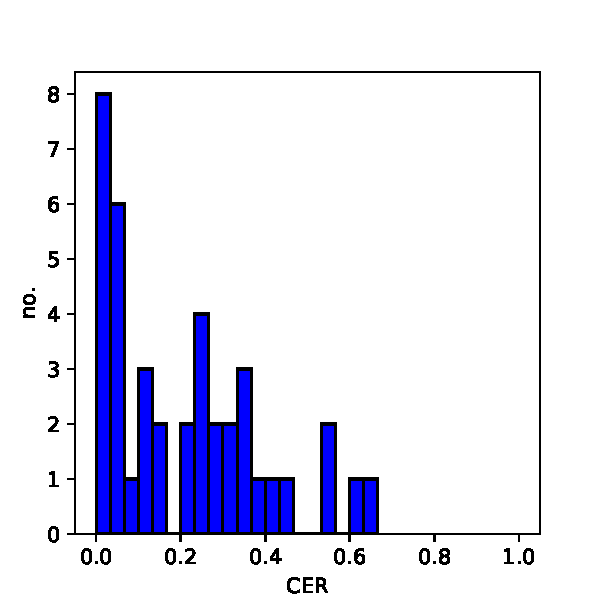
\includegraphics[height=7cm, keepaspectratio]{img/evaluation/CER_on_recognized_words-stage3.pdf}
            \caption{CER dist. on detected words}
            \label{fig:CER_on_recognized_words-stage3}
    \end{minipage}\hfill
\end{figure}

\section{Overall Evaluation}\label{section:evaluation-overall}

The pipeline created consists of 3 stages which take in total an average of 16.07 seconds or 5.9 seconds without the last stage that could not be exactly measured. The average time for processing an image and extracting its text is difficult to be compared to the other works \cite{article:1} \cite{site:0} because of the the differences in hardware, input size and the lack of a standardized benchmark.

However, in terms of performance, we can measure our results with the other works in the field only in averages. My pipeline, before reaching the OCR step, is able to parse 61.74\% of the dataset. This means that in 61.74\% of cases it is able to identify in an image the DOT code and the E-mark (with the mentions specified in section \ref{section:evaluation-text_detection} regarding incomplete detections). This is comparable to the average precision of 64.7\% obtained by \cite{site:0} in the text detection stage, though it must be mentioned that they are interested in tire-markings containing specifications about the tire rather than the identification codes.

If the image that is being processed by my pipeline is not blurry, the OCR provided by Microsoft Cognitive Services \cite{site:Microsoft_Cognitive_Services-Read_API-OCR} is able to recognize the text in the image with an CER of 0.26. The performance on the entire dataset when the blurry images are introduced is lower, the CER reaching 0.51. This is still comparable to the average CER of 0.39 obtained by \cite{site:0} on all tire-markings they were interested in. The work of Kazmi et alia \cite{article:1} obtained an average CER of 0.23 on the 9 images they hand picked and tested on.
